\documentclass[12pt,a4paper]{article}

\usepackage{fullpage}
\usepackage[utf8]{inputenc}
\usepackage{amsfonts}
\usepackage{amssymb}
\usepackage[french]{babel}
\usepackage[cyr]{aeguill}
\usepackage{natbib}
\usepackage{graphicx}
\usepackage{tabularx}
\usepackage{hyperref}
\usepackage[document]{ragged2e}
\setlength{\parindent}{2em}
\setlength{\parskip}{1em}

\newcommand{\quotes}[1]{``#1''}

\begin{document}

\begin{titlepage}
\centering
{\scshape\LARGE Université de Bordeaux \par}
{\scshape\Large Master 1 Informatique  \par}
\vspace{3cm}

{\Huge\bfseries Projet de Programmation\par}
{\Huge\bfseries Le Clicodrome de LEFFF \par}
{\Large\bfseries par Lionel CLEMENT \par}
\vspace{0.5cm}
{\Large\itshape Mémoire \par}
{\large 4 Avril 2019\par}

\vfill
réalisé par \par
BAKIR \textsc{Fatima Ezzahra} \par
JELLITE \textsc{Oumayma} \par
NEDELEC \textsc{Guillaume} \par
SYLLA  \textsc{Alfred Aboubacar} \par
\vfill

{\large Enseignants responsables : Philippe NARBEL et Vincent PENELLE\par}

\end{titlepage}

\newpage
\tableofcontents
\newpage
\listoffigures

\newpage
\tableofcontents
\newpage
\listoffigures

\newpage\section{Introduction}

\subsection{Résumé}
 Ce présent document est le rapport de projet de programmation effectué au sein du Master 1 à l'université de bordeaux.Il décrit les différentes étapes suivies afin de rendre notre projet  \textbf{"Le Clicodrome de LEFFF "} effectif.

 Les objectifs de notre projet consiste à la création d'un site Web interactif permettant de donner accès
au lexique LEFFF pour l'enrichir, et d'analyser un mot donné afin de générer ses formes fléchies à l'aide  d'un interpréteur PFM codé en PHP.
Les interfaces graphiques doivent fournir aux utilisateurs la possibilité d'ajouter, modifier et supprimer les mots, les règles ect... .
Il permettent également de proposer les différents formes fléchies de n'importe quel mot. Ainsi, des interfaces pour l'exportation et l'importation du lexique. 

Pour réaliser ce projet , nous choisissons l’implémenter en PHP, en utilisant le framework Symphonie pour le site Web et MySQL pour la base de données.
\subsection{Contexte}

\smallbreak 

Notre client Lionel Clement a réalisé un lexique des formes fléchis du Français "LEFFF"  contenant un grands nombre de mots de différentes catégories. Cependant, ce lexique est présenter sous format texte et il n'existe pas d'outils permettant de faciliter son accès,sa modification et son enrichissement.Le système actuel n'assure pas une bonne traçabilité des modifications des mots effectués par les linguistes et ne permet aucun contrôle de ces modifications.

Pour cela , il serra donc utile de concevoir un site Web interactif qui va permettre de donner accès au lexique pour l'enrichir et l'extraire , et d'implémenter un outil qui va générer le formes fléchis .

/********** AUTRE PROPOSITION ************/
Lionel CLEMENT est un enseignant-chercheur du Labri (Laboratoire Bordelais de Recherche en Informatique) informatique, spécialisé dans le domaine de la linguistique formelle et du traitement automatiques des langues. Il a réalisé avec Benoît SAGOT, chercheur dans le même domaine à l'Inria (Institut National de Recherche en Informatique et en Automatique), le Lexique des formes fléchies du français, appelé le LeFFF.

Aujourd'hui, ce lexique n'est disponible que dans un fichier au format texte, ce qui ne facilite pas sa consultation, sa modification ou son enrichissement.

\subsection{Objectif}

Avant de détailler l'objectif de notre projet, nous allons mettre
au clair quelques notions nécessaires à la compréhension du sujet. 
D'abord dans la langue française, les formes fléchies d'un mot correspondent à sa conjugaison et à ses déclinaisons (sa forme au pluriel, les mots ayant une correspondance comme "mien" et "moi" par exemple).\\
Ensuite,pour la génération des formes fléchis nous allons utiliser le formalisme PFM (Paradigm Function Morphology),selon cette approche , l'association d'un mot  fléchi avec ses propriétés morphosyntaxiques permet d'appliquer des règles déterminant la forme flexionnelle de ce mot .\\
De plus ce lexique est un “dictionnaire” contenant un grands nombre de mots de différentes catégories. Ce sont des noms propres, des noms communs, des adverbes, des adjectifs, des tous les autres types de mots possible dans la langue française. 

Notre but sera de trier tous ces types de mots afin de déterminer quelles sont les formes fléchies et quelles sont les mots "racines".

Lionel CLEMENT qualifie ce lexique comme "une ressource complexe constituée de
\begin{itemize}
\item Lexème ou grammème (ie Prendre)
\item Vocables (ie Prendre=saisir, Prendre=recevoir)
\item Catégories syntaxiques (ie Verbe)
\item Sous-catégories syntaxiques (ie Transitif, passivable)
\item Catégories grammaticales (ie Nombre$\rightarrow\{sing, plur\}$, Personne$\rightarrow\{1, 2, 3\}$)
\item Règles de flexion (ie Table de conjugaison de prendre - Stem=.*(pren|mett))
\item Valence (ie objet nominal, oblique en à)
\item Réalisation syntaxique (ie passif en par)
\item Phraséologie (ie "Prendre ombrage", "Prendre ses jambes à son cou")
\item Collocation (ie "Prendre une initiative")
\item Fonctions lexicales (ie Magn: "Prendre une belle initiative")
\end{itemize}

L'objectif de ce projet est donc de transformer le lexique au format texte en une base de données et de développer une interface Web facilitant les interactions avec ce lexique via cette base de données.
Le projet peut être donc séparé en trois parties principales : 
\begin{itemize}
    \item L'importation du lexique au format texte dans une base de données
    \item La création de l'interface web qui interagira avec la base de données
    \item Le développement d'un interpréteur permettant de générer les formes fléchies d'un mot donné en entrée .
\end{itemize}
\subsection{Analyse de l'existant}
\subsection{Le lexique LeFFF }
Pour ce projet, nous avons a notre  disposition différentes versions  du Lefff  dont la dernière réalisé par Benoît Sagot en 2010. Cette version regroupe diffèrent format du lefff , à savoir \cite{lefff_int} :
\begin{itemize}
\item le lexique \textbf{intentionnel}, qui décrit pour chaque entrée son lemme (forme canonique + tableau d'inflexion) ainsi que des informations syntaxiques profondes (cadre de sous-catégorisation profonde + réalisations possibles + restructurations possibles) .
\item le lexique \textbf{extensionnel}, construit automatiquement par compilation du lexique intentionnel. Ce processus de génération comprend une étape d'inflexion, en fonction de la classe d'inflexion associée à l'entrée intentionnelle, puis une étape de construction des différentes structures syntaxiques (une pour chaque restructuration pertinente) associées à chaque forme infléchie (les informations syntaxiques peuvent varier d'une forme à une autre, notamment les formes infinitive, de participant, d'une restructuration à une autre).
\end{itemize} 

\smallbreak Les formats de la dernière version de lefff ont des extensions et contenues différents, le lexique \textbf{intentionnel} est manipulable grâce à l'outil "alexina-tools" qui permet de le compiler pour avoir le format extensionnel avec seulement les paramètres morphologiques et une avec tous les paramètres d'un mot .

Le lexique extensionnel avec seulement les paramètres morphologiques est présenté sous la forme ci-dessous :
\begin{verbatim}
démariés	adj	démarier	Kmp
démariés	v	démarier	Kmp
démarqua	v	démarquer	J3s
démarquage	nc	démarquage	ms
démarquages	nc	démarquage	mp
\end{verbatim}

\smallbreak La première colonne comprend le mot recherché. 
\smallbreak La seconde présente sa catégorie (\textbf{adj}(adjectif), \textbf{v}(verbe), \textbf{np}(nom propre), \textbf{nc} (nom commun).
\smallbreak La troisième colonne présente le mot auquel est lié le mot de la première colonne.
Si la première colonne et la troisième sont différentes, cela signifie que le mot de la première colonne est une forme fléchie du mot de la troisième colonne. S'il les 2 colonnes sont identiques alors c'est que ce mot est un mot que l'on sauvegardera dans la base de données avec ses attributs.
Enfin la dernière colonne apporte des informations sur le mot comme le genre, s'il est singulier pluriel ou encore a quel personne le verbe est employé. Une explication de ces codes est disponible sur le site de Lionel CLEMENT \cite{tagset}.

La différence entre le contenu des différents formats de fichier du LeFFF à notre disposition est principalement le détail par rapport au paramètre morphologique du mot.
\subsection{Le formalisme PFM  }
      Le format de base des règles : \textbf{n, Xc, t -> f(X) } \\
\begin{itemize}
    \item n : l’ordre de priorité pour l’application des règles
    \item X : la racine du lexème.
    \item C : la classe du lexème (sa catégorie).
    \item t : règles à appliquer
    \item f(X) : la forme flexionnelle
\end{itemize}

Exemple de règles pour les adjectifs : \\
\textbf{1, racine,{f} -> racine + "ne"} \\
\textbf{2, racine, {p}-> racine + "s"}

Exemple d'application : \\
PF(Sien, {f,p} ) = 2 o 1(Sien, {f,p} )(\textbf{ epsilon}) \\
                 = 2(Sien, {f,p} )(\textbf{ Sienne}) \\
                 =\textbf{ Siennes }

Pour cet exemple on veut mettre le mot sien au féminin pluriel ; la première règle à appliquer c'est d'ajouter le "ne" du féminin puis ajouter le "s" du pluriel en appliquant la deuxième règle ce qui nous assure l'ordre de priorité d'application des règles pour ne pas avoir des incohérences .à savoir \cite{PFM} :

\section{Analyse des besoins}
\subsection{Analyse des besoins fonctionnels}
\smallbreak Lors de nos communication avec le client, nous avons pu identifié ses principaux besoins pour le projet. En effet, le projet se découpe en trois partie principales : 
\begin{itemize}  
  \item Une application web permettant aux utilisateurs d'interagir facilement avec le lexique
  \item une base de données contenant les différents mot du lexique (les formes fléchies des mots sont exclus de la base) et leurs attributs.
  \item Un interpréteur PFM permettant, pour un mot donné, de générer ses formes fléchies.
\end{itemize}

\smallbreak Pour apporter un contrôle des interactions des utilisateurs depuis le site web, un système de rôle sur le site sera mis en place. Avant de présenter la liste des besoins fonctionnels identifiés, voici une présentation de ces différents rôles, qui vous aidera a mieux comprendre ces besoins : 
\begin{itemize}  
  \item \textbf{Les visiteurs} : Ils ne peuvent que rechercher, consulter les mots du lexique, signaler des erreurs sur un mot ou exporter le lexique.
  \item \textbf{Les éditeurs} : Ce type d'utilisateur peut, en plus d'avoir les mêmes droits que les visiteurs, modifier (le mot ou ses attributs) un mot du lexique. Ces actions ne peuvent être effectué qu'en étant connecté (système d'authentification) sur le site.
  \item \textbf{Éditeur Expert} :  Ces utilisateurs sont des éditeurs pouvant supprimer des mots du LeFFF et qui peuvent ajouter des catégories.
  \item \textbf{Les administrateurs} : Ils ont un contrôle total de l'application. En plus d'agir comme des modérateurs, ce sont qui valident les inscriptions sur site, gèrent les rôle des différents utilisateurs et ont le pouvoir de bannir des utilisateurs du site.
\end{itemize}
 \subsection{Gestion du lexique LeFFF}
\textbf{Importer le LeFFF dans une base de données relationnelle}


\textbf{Priorité : 1} \\ 
Cette fonctionnalité permet d'importer les données du lexique dans un format donné (.txt / .mlex) directement dans une base de données où l'architecture sera préalablement configuré.
Cette fonctionnalité est nécessaire pour alimenter notre base de donnée puisque le leFFF comprend un très grand nombre de données (environ 500 000 lignes).
Pour l'implémenter, nous allons définir un algorithme qui permet de découper le fichier d'entrée, de filtrer les mots a enregistré et d'effectuer des requêtes d'ajout dans notre base de données


 \textbf{ Exporter le Lefff} 
 
 
\textbf{Priorité : 3}  \\
Tous les utilisateurs peuvent effectuer une exportation du lexique. Cette option sera disponible depuis notre application web. Cette opération nécessite l'utilisation du compilateur PFM pour générer les formes fléchis de tous les mots présents dans la base de données.
Nous proposerons aussi une exportation du lexique sans les formes fléchies, qui sera bien plus rapide et légère.
\subsection{Gestion du mot} 
\textbf{Rechercher un mot}


 \textbf{Priorité : 2}
\\ Nous avons mis à la disposition de tous les utilisateurs un champ de saisie sur toutes les pages de l'application web leur permettant de rechercher un mot. A la manière d'un moteur de recherche classique, la liste des mots enregistrés dans notre base de données, correspondant plus ou moins à ce qui a été recherché apparaîtront sur la page. Il sera ensuite possible à l'utilisateur de consulter en détail un mot, de signaler une erreur, de le modifier ou le supprimer (Si les droits de l'utilisateur le lui permet). Si aucun mot ne correspond en base de données, un message d'avertissement apparaîtra sur l'interface.


\textbf{Consulter un mot} 


 \textbf{Priorité : 2}
\\ Tous les utilisateurs du site web peuvent consulter un mot. Pour cela il suffit à l'utilisateur de rechercher un mot (voir la partie "Rechercher un mot") et de sélectionné le mot voulu. Ce mot sera ensuite envoyé à notre interpréteur pour générer ses formes fléchies et les renvoyer à notre application afin d'avoir toutes les informations du mot affichées sur l'interface.
Si les droits de l'utilisateur le permet, les boutons d'ajout, de modification et de suppression apparaissent sur cet écran.


\textbf{Ajouter un mot} 


 \textbf{Priorité : 2}
\\ Cette fonctionnalité est réservé au utilisateurs authentifiés (les administrateur ,les éditeurs et les modérateurs). Un formulaire est proposé, où il est demandé d'ajouter le mot, ses catégories (adjectifs, nom commun etc...), et ses tags (par exemple groupe pour les verbes)
Avant d'ajouter le mot en base, des vérifications seront effectués afin  de vérifier si le mot n'existe pas déjà en base, ou si le mot n'est pas une forme fléchies d'un mot en base de données.


\textbf{Supprimer un mot} 


 \textbf{Priorité : 2} \\ 
 Les modérateurs et les administrateurs peuvent supprimer un mot de la base de données. Il suffit simplement de rechercher le mot et d'appuyer sur "Supprimer". Une notification sera envoyé aux administrateurs pour les informer de la suppression du mot. Le mot sera alors supprimé de la base de données.

\textbf{Modifier un mot} 


 \textbf{Priorité : 2} \\ 
 La fonction de modification d'un mot ressemble à celle d'ajout (voir partie Ajouter un mot). Elle est accessible a tous les utilisateurs connectés. En effet le formulaire sera le même mais pré rempli avec les informations existante du mot. Il suffit à  l'utilisateur d'effectuer les modification qu'il souhaite et de les valider pour que les changements soient enregistrés dans la base de données.

\textbf{Signaler un mot} 


 \textbf{Priorité : 2}
 \\ Les visiteurs simple et les éditeurs ont la possibilité de signaler des erreurs sur un mot. Ce mécanisme permet d'envoyer une notification aux administrateurs pour leur faire part d'informations sur un mot en particulier. 
 \subsection{Génération des formes fléchis} 
 
 
 \textbf{Priorité : 1} \\
Pour répondre a cette fonctionnalité nous avons mis en place un interpréteur qui permet de générer les formes fléchies d'un mot.
En effet, Le rôle de l'interpréteur est important lors de la consultation d'un mot et l'exportation du lexique.Pour la recherche du mot l'utilisateur doit données en paramètre le mot, dans un premier temps , on récupère les règles , les tags du mot et les combinaison de tags qui convient avec la catégorie du mot donnée en entrée, ensuite on filtre les règles selon la correspondances avec les tags du mot et on récupère aussi les règles définissant le radical du mot sachant que nous avons choisi de stocker pour chaque mot une règle qui définit son radical avec le formalisme PFM ,puis en vérifie si le tag du mot est renseigne dans les règles et si le mot en lui-même est un tag de la règle . 
Dans un deuxième temps on vérifie si tous les tags de la règle sont renseignes dans la combinaisons ou si aucun tag n'est renseigné ensuite on fait un tri des règles dans leur ordre d'application .
Pour l'application des règles on vérifie au début si la règle possède une combinaison de tags correspondant à une combinaison de tag de la catégorie si c'est le cas on l'applique, sinon on l'ignore en plus si plusieurs règles s'appliquent pour une combinaison données , elles respecte l'ordre croissant du niveau d'application.

 D'aprés le formalisme PFM une règle a des niveaux, et le premier niveau de chaque règle est 0 'la détermination du radical'.Si on a deux règles  avec le même niveau, la règle la plus spécifique avec le plus de tags qui correspondent s'applique et on ignore les autres . Pour l'ordre de priorité, il s'applique quand on aura des priorités dans la langue et on doit appliqué une règle avant l'autre. 
\subsection{Gestion des règles } 


 \textbf{Priorité :  1} 
 
 
\textbf{Ajouter une règle }  \\ Seulement les utilisateurs ayant le droit de gérer les règles qui peut ajouter ces règles à partir d'une interface où il est demandé d'ajouter la catégorie , le niveau d'application de la règle et l'ordre de priorité de cette règle,les tags liés aux mot et les tags d'application de la règle. Dans le cas d'un  verbe, le radical du mot doit être ajouter dans la même interface.Enfin le résultat de la règle avec un champs préfixe,mot et suffixe.
Avant d'ajouter la règle en base, des vérifications seront effectués afin  de vérifier si la règle n'existe pas déjà en base.

\textbf{Modifier une règle } \\ Comme pour la modification du mot nous avons repris le même formulaire d'ajout pré-rempli avec les informations existante de la règle . L'utilisateur doit juste effectuer les modification qu'il souhaite et de les valider pour que les changements soient mise à jour  en base de données.


\textbf{Supprimer une règle }  \\ Pour la suppression le site web doit fournir aux utilisateurs une liste des règles. Il suffit de rechercher la règle et d'appuyer sur supprimer, la règle  sera alors supprimé de la base de données.

\subsection{Gestion des combinaisons de tags } 
 \textbf{Priorité : 1 } 
 
 
\textbf{Ajouter une combinaison } \\ Les combinaisons de tags  sont  toutes les tags qui convient avec la catégorie de chaque mot, ces combinaisons sont géré par les utilisateurs qui doivent les ajouter d'une façon cohérente.
Pour les ajouter, un formulaire est mis en place pour ajouter la catégorie du mot et les combinaisons. Avant d'ajouter la combinaison de règle en base, on vérifie si la combinaison n'existe pas déjà en base.

\textbf{Modifier et Supprimer une combinaison }  \\ Comme pour la modification et la suppression d'un mot ou d'une règle nous avons mis en place une liste des combinaisons avec des boutons supprimer et modifier .

 
\subsection{Gestion des catégories } 
 \textbf{Priorité : 2 } \\
\textbf{Ajouter une catégorie } \\ Cette fonctionnalité  est mis en place pour que les utilisateurs concernés peuvent ajouter des catégories . Le formulaire propose contient les champs suivant : le code de l catégorie et sa valeur (exemple : code v , valeur verbe ).

\textbf{Modifier et supprimer  une catégorie } \\ Pour cette fonctionnalité aussi nous avons propose une liste de catégorie avec des boutons supprimer et modifier .
\subsection{Généralité de l'interpréteur} \textbf{Priorité : 1}\\ cette fonctionnalité est mis en place pour que l'interpréteur soit générique et qu'on puisse générer les formes fléchis de n'importe quel mot dans n'importe quelle langue . Pour cela nous avons fait un choix spécifique pour l'organisation de notre bases de données qu'on va l'expliquer plus tard dans la partie architecture .

\subsection{Contrôler les interactions } 
 \textbf{Priorité : 2}
\\ Tous les utilisateurs doivent d'authentifier pour pouvoir modifier où enrichir le LeFFF. Afin d'ajouter de la sécurité, nous avons décider de mettre constamment des message de validation pour être sur que l'utilisateur souhaite réellement effectuer une action et ne pas faire d'erreur.
De plus un système de déconnexion automatique après une période d'inactivité (environ 10 minutes) sera mis en place en cas d'oubli de fermeture de session afin que personne ne puisse subtiliser la session.
Enfin des logs seront implémentés afin de tracer les changements effectués en plus de l'historique.

\subsection{Gestion des rôles:} 
 \textbf{Priorité : 3} \\
Pour qu'un utilisateur puisse effectuer des tâches d'ajout, de modification ou de suppression de mot, il faut qu'un administrateur lui affecte ces droits (les rôle d'éditeur ou modérateur). A cet égard, on doit créer une interface où l'administrateur puisse faire cela.
Sur cette interface, apparaîtra la liste des comptes utilisateurs, pour chaque utilisateur se trouvera des boutons  : \textbf{Supprimer} cet utilisateur ,\textbf{ Modifier} le rôle de cet utilisateur. 
Sur la même interface on va mettre en place un bouton pour \textbf{Valider} l'inscription d'un nouvel utilisateur.


\subsection{Gestion de l'historique d'un mot} 
 \textbf{Priorité : 3} \\
Nous avons décidé de mettre en place un historique permettant d'enregistrer tous les ajouts, modifications et suppression. Pour cela nous allons enregistrer les données modifiées en base de données.
\section{Analyse des besoins non fonctionnels}
\smallbreak

\subsection{Sécurité}
\textbf{Priorité : 1}
\smallbreak
Afin de protéger l'intégrité des données du LeFFF dans la base de données, nous sécuriserons la base et l'application web des problèmes de sécurité suivants :
\begin{itemize}
    \item \textbf{Les injections SQL}, permettant de récupérer ou d'altérer des données, voir même prendre le contrôle de serveur. L'attaque par injection SQL consiste à injecter du code malicieux SQL qui sera interprété par le moteur de base de données dans un champ de saisie d'une application web. \\
    \textbf{Notre solution :} Afin de se protéger de se genre d'attaque, nous avons choisi de développer l'application web en PHP avec le framework Symfony, qui comprend un l'ORM (Object-Relational Mapping) Doctrine. Cet ORM est une couche d'abstraction de base de données qui permet d'interagir avec le contenu de la base de données en manipulant des objets (informatique) du coté de notre application. Il comprend des modules de sécurité (génération de contraintes, formatage des données envoyées ect...) qui détecte les attaques par injection SQL.
    
    \item \textbf{Le Cross-Site Scripting (XSS)} : Cette faille permet d'injecter du code malicieux sur une page web. Par exemple sur un forum, si quelqu'un entre en commentaire un code Javascript nuisible, tous les autres utilisateurs qui accéderont à cette page seront impacté par ce code qui s'exécutera sur leur navigateur. \\
    \textbf{Notre solution :}Pour remédier à cela, le framework Symfony possède aussi un système (filtrage des données d'entrées, échappement des données en sortie...) protégeant de ce genre d'attaque afin de filtrer tous ce qui pourrait ressembler à du code. C'est un procédé assez similaire à celui de la protection contre les injections SQL.
    
    \item \textbf{La falsification de requête inter-sites (CSRF)} : Cette faille permet à un attaquant de forcer ses victimes à effectuer certaines actions sur un site cible, sans qu'elles s'en aperçoivent. Pour cela, les attaquants cherche à ce que leur victime visite une page (en étant connecté) où des scripts malicieux seront exécutes sans que la victime s'en aperçoive à l'aide de balise image chargeant le script par exemple. La victime étant authentifié sur le site, les scripts pourront s'exécuter correctement et corrompre les données du site. \\
    \textbf{Notre solution :} Voici la dernière faille de sécurité à laquelle Symfony nous protège. En effet le framework fait cela en générèrant des jetons ("tokens") au moment de l'authentification, différents pour chaque utilisateur et qui sont stockés dans la session. Ce jeton est ensuite vérifié a chaque action avec la base afin de vérifier que c'est bien une action voulue par l'utilisateur et non une attaque CSRF. 
    
    \item \textbf{Le déchiffrement de données} qui consiste à déchiffrer des données crypté. Cela peut permettre de trouver des mot de passe et donc prendre le contrôle d'une session utilisateur ou bien de découvrir des informations sensibles (informations bancaire, personnelles...) \\
    \textbf{Notre solution :} Pour éviter cela, nous avons décidé de chiffrer les données avec des algorithmes irréversible (une fois crypté, aucune technique connue à ce jour peut décrypter le mot, il faut forcement connaître le mot initial) comme "bcrypt" ou "sha512".
    
    \item \textbf{L'écoute de communication réseau} : Requêter un site web avec un protocole HTTP permet à des intrus présent sur votre réseau de lire ou modifier le site internet que vous souhaitez consultez et présente donc un gros risque. \\
    \textbf{Notre solution} : Utiliser le protocole HTTPS qui permet de chiffrer les données échangées et ainsi les protéger de toutes interceptions ou modification.
\end{itemize}

\subsection{Format de fichier}
\textbf{Priorité : 2}
\smallbreak
\begin{itemize}
\item Afin de pouvoir répondre aux besoins d'importation et d'exportation du LeFFF avec la base de données, il nous faut définir les format de fichiers compatibles avec ces fonctions.
Nous avons fait le choix d'utiliser les formats textes et elex (.txt et .elex)  car ce sont les formats disponibles au téléchargement du LeFFF actuellement. Ce choix nous permet de pouvoir exploiter le LeFFF existant sans avoir à le reformatter dans un autre format.
\end{itemize}

\subsection{Performances}
\textbf{Priorité : 3}
\smallbreak
Au niveau des performances, nous avons décider de faire une implémentation du projet de manière à ce que la requête de demande des formes fléchies d'un mot (requête en base et génération des formes fléchies par le compilateur) n'excède pas les deux secondes d'exécutions. De plus les actions d'importation et d'exportation étant plus lourdes, nous voulons implémenter ces fonctions pour qu'elles n'excèdent pas 10 minutes d'exécution.

\subsection{Ergonomie}
\textbf{Priorité : 4}
\smallbreak
Nous avons fait le choix d'adopter une design très simple et épurée afin que l'utilisateur ne se perde pas dans l'interface et puisse trouver des solutions à son besoin de manière simple et naturelle.
\smallbreak
Des codes couleurs et icônes distinctifs seront mis en place afin que l'utilisateur comprennent le plus rapidement possible à quoi il est confronté. (par exemple, les messages en rouge correspondront à des messages d'erreurs, le vert pour la validation et du jaune pour des avertissements.).

\subsection{Solutions proposées : les besoins réalisés}

Après l'analyse des problèmes du système actuel, nous avons proposé la réalisation d'un site Web  adaptée aux besoins 
qui permettra d'améliorer le processus de travail et de gagner plus de temps en assurant :

\begin{itemize}
\item \textbf{Importations des fichiers} : Intégration à partir d'une interface graphique, le lexique qui existent dans l'archive du format texte.
\item \textbf{Exportations des fichiers} : Pour avoir une versions de lexique sous format texte.
\item \textbf{Recherche} : Pour avoir une version de lexique sous format texte.
\item \textbf{Gestions des données} : d'une façon rapide et efficace et dans une seule interface graphique.


\item \textbf{L'ajout des mots, des règle, des combinaisons et des catégories.}


\item \textbf{ La modification et la suppression des mots, des règle, des combinaisons et des catégories.}
\item \textbf{Intégration d'un interpréteur PFM } : qui permet de générer les formes fléchie lors de la consultation des mots et l'exportation du lexique.
\item \textbf{Possibilité du filtrage} : lors de la recherche dans les listes.
\item \textbf{Possibilité de la modification et suppression dans les listes.}
\item \textbf{La généralité de notre interpréteur} : En effet nous avons fait en sorte que notre interpréteur soit générique pour pour pouvoir générer des formes fléchis de n'importe quel mot dans n'importe quel langue , d'ailleurs nous avons fait un exemple sur la langue perse .
\end{itemize}


\subsection{Les besoins non réalisés : Faute de temps}

On a pas réussi à implémenter les  fonctionnalités suivantes:

\begin{itemize}
\item \textbf{La protection des données } : A l'aide d'une page d'authentification.
\item \textbf{La gestions des rôles }
\item \textbf{Le signalement d'un mot}
\item \textbf{La gestion de l'historique}
\end{itemize}


\section{Architecture et description du logiciel}
\subsection{Architecture de la base de données }
\begin{figure}[h]
\centering
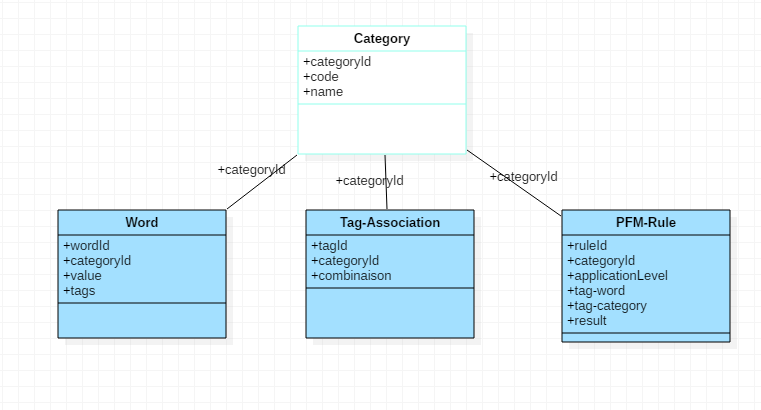
\includegraphics[width=150mm]{img/basefinal.PNG}
\caption{Architecture: Base de données}
\label{Tux}
\end{figure}

Notre base de données est constitué de quatre tables : 
\begin{itemize}
\item \textbf{Category} : Cette table contient le code et le nom de la catégorie ,par exemple code : adj et name : adjectif .
\item \textbf{Word} : La table word contient une référence categoryid vers la table category , la valeur du mot et ses tags (exp : groupe,etc).
\item \textbf{Tag-Association} : Cette table contient des combinaisons de règles qui marche avec une catégorie renseignée par la clé étrangère CategoryId  et un tag du mot par exemple le groupe pour les verbes en français .
\item \textbf{PFM-Rule} : Nous avons choisi de stocker les règles PFM en base pour pouvoir les récupérer facilement par la suite et générer les formes fléchis d'un mot , en plus nous avons mis en place une interface pour que l'administrateur ou l'éditeur puisse ajouter des règles .

\end{itemize}



Nous avons choisi cette organisation de base de données pour pouvoir générer des formes fléchis de n'importe quelle langue .En effet nous avons pas spécifié les tags du mot a stocker dans la base ça peut être "groupe" pour les verbes de français ou " irregular verb " pour les verbes en anglais .



\subsection{ Architecture du Site Web }
\subsection{Architecture du site} 

\begin{figure}[h]
\centering
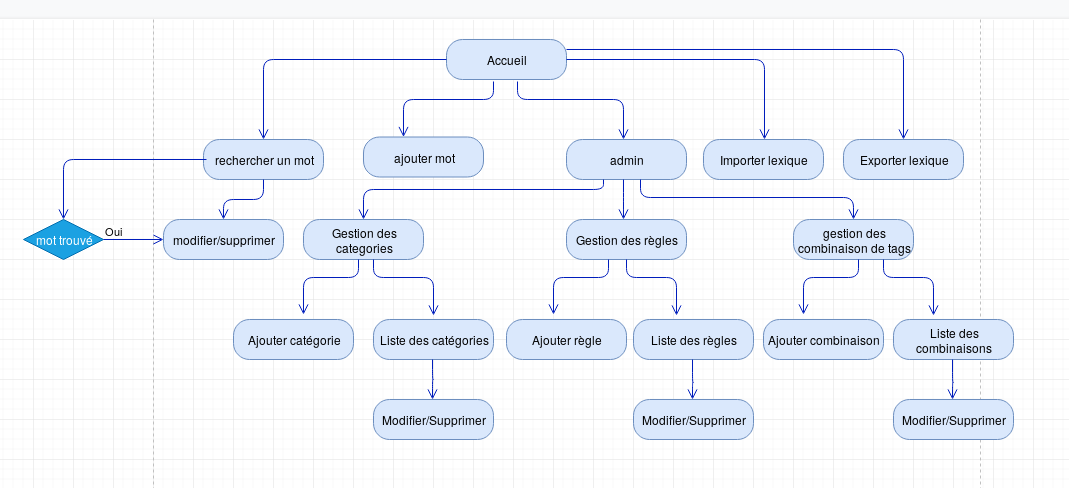
\includegraphics[width=150mm]{img/site1.png}
\caption{Architecture: Site web}
\label{Tux}
\end{figure}


Nous avons réussi à mettre en place les interfaces décrit dans le schéma ci-dessus,
notre site web est réalisé seulement pour l'administrateur, qui doit s'authentifier
avant d'accéder aux différents services proposé par le site.

Cette interface permet aux utilisateurs de s'authentifier à l’aide d'un login et un Mot de passe, 
et faire la redirection vers la page d'accueil (dans notre application la page d'accueil
pour l'administrateur c'est le page de recherche d'un mot).

La recherche d'un mot consiste à afficher toutes les formes fléchies qui lui correspond. Une fois ces formes sont affichées, 
l'administrateur peut modifier le mot qu'il vient de rechercher.

La page d'accueil contient également des boutons qui redirigent vers les différents interfaces d'ajout : 
\begin{itemize}
    \item   Ajouter règle
    \item   Ajouter mot
    \item   Ajouter combinaison
    \item   Ajouter catégorie
   \end{itemize}
et elle redirigé aussi aux  pages qui permet d'importer ou d'exporter le lexique.

\newpage
\subsection{Exemple de bon fonctionnement: Interfaces} 

  \textbf{ Rechercher Mot }

Les utilisateurs peuvent consulter la liste des formes fléchies du mot comme vous voyez dans cette interface :


\begin{figure}[h]
\centering
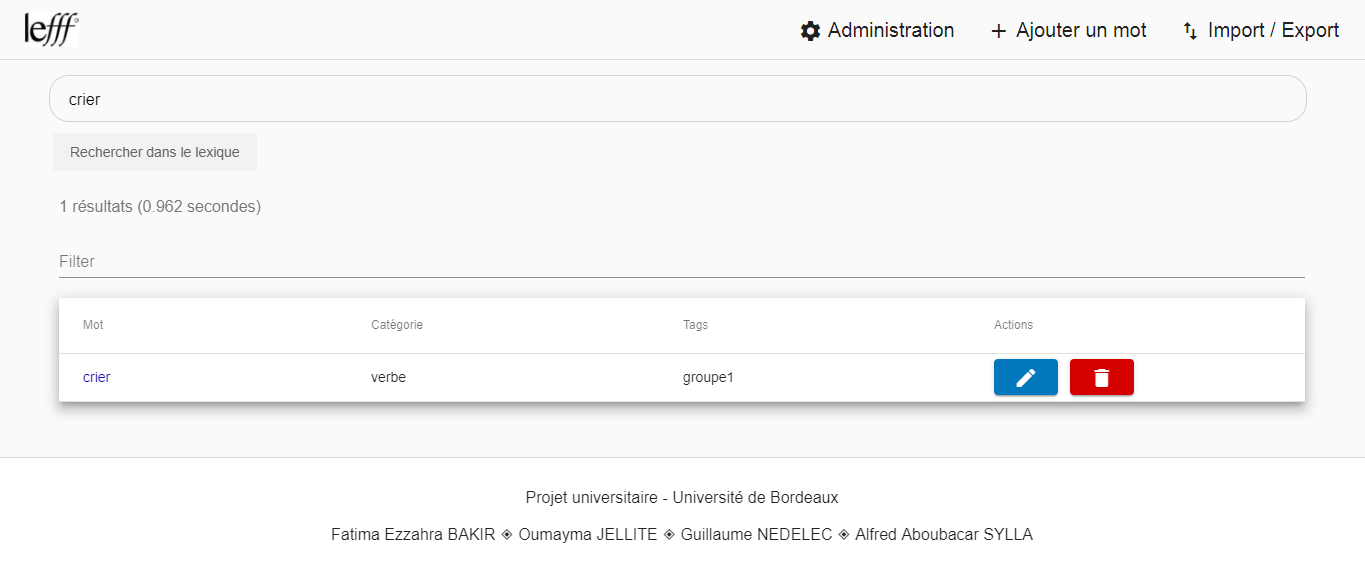
\includegraphics[width=150mm]{img/Recherche.PNG}
\caption{Interface: Rechercher mot}
\label{Tux}
\end{figure}




L’utilisateur (l’administrateur) peut gérer le mort en le modifiant ou le supprimer.


  
  \textbf{ Ajouter mot}


L'administrateur a le droit d'ajouter des nouveaux mots  en accédant à l'interface suivante: 


\begin{figure}[h]
\centering
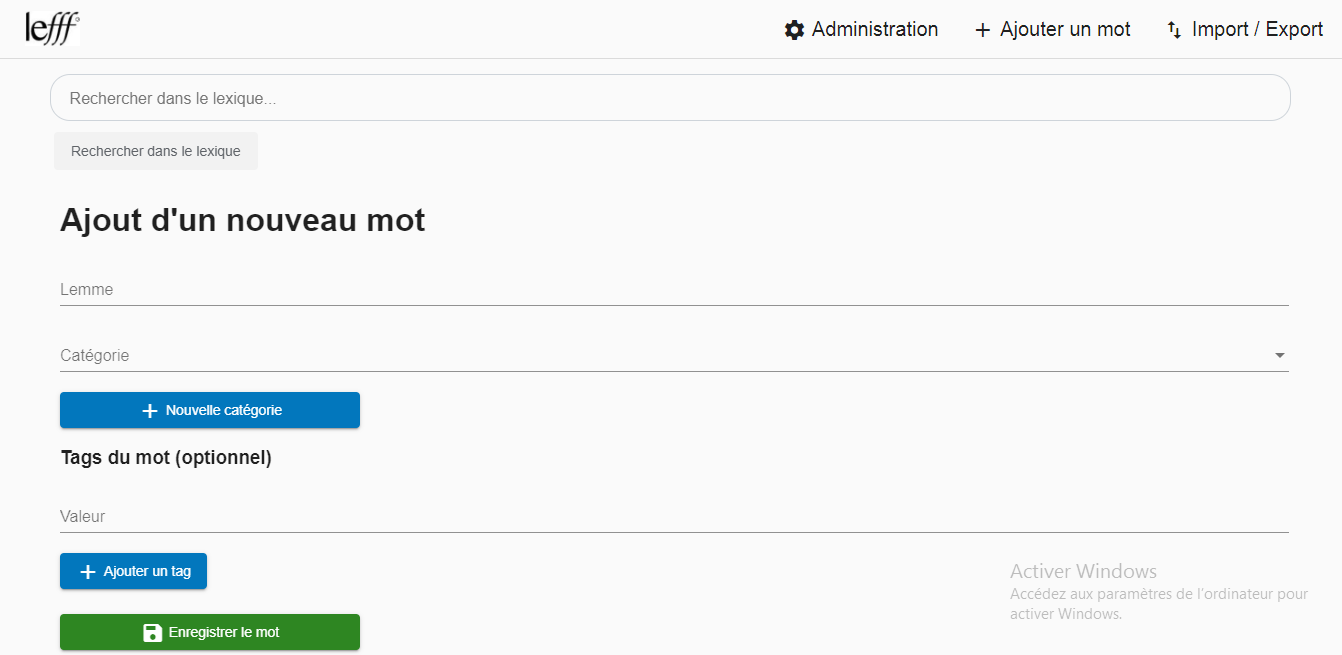
\includegraphics[width=150mm]{img/Ajoutermot.PNG}
\caption{Interface: Ajouter mot}
\label{Tux}
\end{figure}


Si le mot  est ajouté, un message de réclamation s'affiche. Une fois il est ajouté, l'utilisateur peut cliquer sur les boutons "Modifier" ou "Supprimer" si il a commis une erreur comme le montre la figure suivante:



 
\textbf{Éditer un mot}
\begin{figure}[h]
\centering
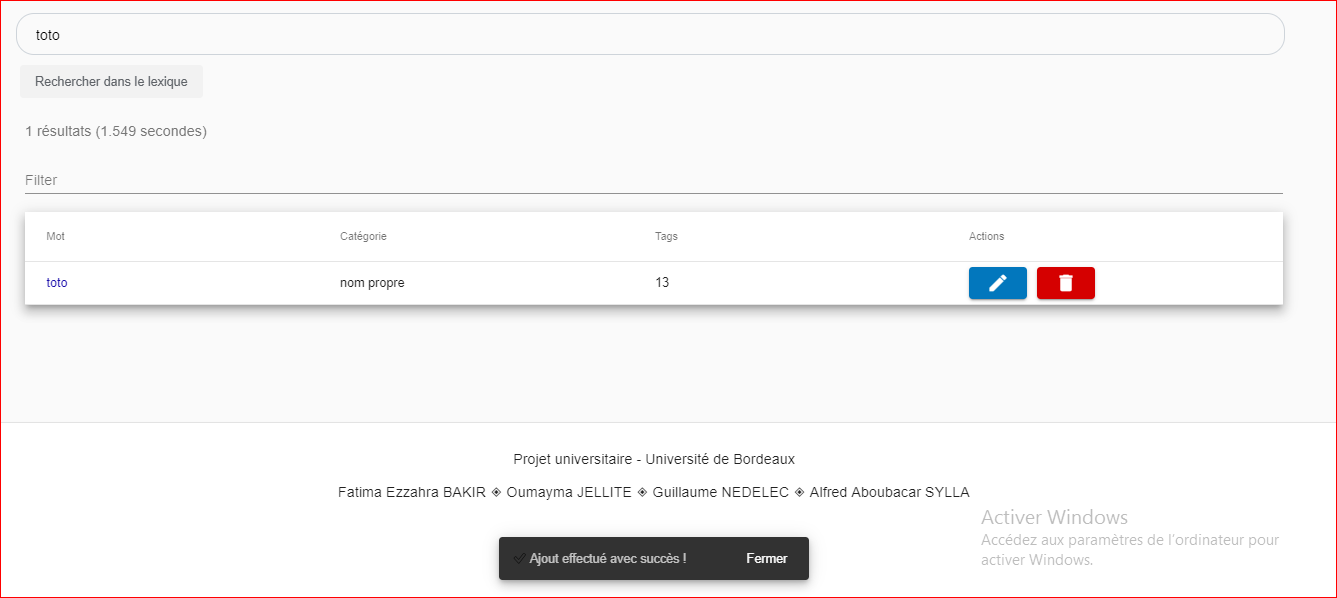
\includegraphics[width=150mm]{img/AjoutEffectuer.PNG}
\caption{Interface: Ajouter mot}
\label{Tux}
\end{figure}

comme vous pouvez le voir sur la figure ci-dessus nous avons mis en place une interface pour pouvoir éditer un mot ; modifier ,supprimer et consulter un mot juste en cliquant sur les boutons présente sur l'interface .
Nous avons fait la même chose pour la gestion des règles et les combinaisons de tags .

 
   \textbf{Exporter le lexique}

Les utilisateurs peuvent aussi exporter le lexique en extrayant tous les mots enregistrés en base de données dans l'ordre alphabétique avec leurs formes fléchies générer par l'interpréteur :
Les formes fléchies de chaque mot seront généréés sont presentés dans l'export à la suite du mot correspondant en respectant le format ci-dessous :\\
\textbf{<mot> <code-catégorie>["<categorie-name">] lemme="<mot>" {<mot-tags>}} \\
\textbf{<forme-fléchie-générée>  f["forme fléchie"] lemme="<mot>" {<tags-combinaison>}}\\
\textbf{<mot> <code-catégorie>["<categorie-name">] lemme="<mot>" {<mot-tags>}} \\
\textbf{<forme-fléchie-générée>  f["forme fléchie"] lemme="<mot>" {<tags-combinaison>}}\\
\textbf{<forme-fléchie-générée>  f["forme fléchie"] lemme="<mot>" {<tags-combinaison>}}\\
...

\begin{itemize}  
\item \textbf{mot} : mot de la base .
\item \textbf{code-catégorie} : le code de la catégorie du mot 
\item \textbf{catégorie-name} : le nom complet de la catégorie.
\item \textbf{mot-tags} : les tags renseignés sur le mot . Chaque tag est séparé par un ";".
\item \textbf{forme-fléchie-générée} : une forme fléchie du mot présentés précédemment
\item \textbf{f["forme fléchie"]} : "f" correspond au code de la forme fléchie. 
\item \textbf{lemme="<mot>"} : avec <mot> correspondant au lemme de la base de la forme fléchie .
\item \textbf{<tags-combinaison>} : l'association de tags ayant permis de générer la forme fléchie .Chaque tag est séparé par ";".
\end{itemize}

 
  \textbf{ Importer le lexique}

ON a ajouté une interface ou les utilisateurs peuvent importer les fichier sous format texte qui existent déjà. Pour cela on a définie 3 syntaxes différentes : 
\begin{itemize}

  \item La  première correspond à celle respectée par notre fonctionnalité d'export.
  \item La deuxième  correspond à la syntaxe du Lefff consultable le site de Lionel CLEMENT.
  \item Et La troisième  correspond à la syntaxe du Lefff au format .mlex consultable sur le site de Benoît SAGOT..
\end{itemize}

\subsection{Outils de développement}

Ce projet est divisé en 3 parties :
\begin{itemize}  
  \item l'application web
  \item l'interpréteur
  \item la base de données
\end{itemize}

\textbf{Application web et L'interpréteur : PHP avec le framework Symfony 4:}

Nous avons choisi de développer le site Web et l'interpréteur en PHP car c'est un langage simple d'utilisation et que ce framework apporte beaucoup d'avantages en termes de sécurité (comme énoncé précédemment dans la partie 2.2.1) et de développement (configuration simple et rapide ect...) ainsi, qu'il offre des 

\smallbreak

\textbf{Base de données : MySQL:}


Pour la base de données, le choix s'est porté sur MySQL pour sa facilité d'utilisation et sa bonne compatibilité avec le framework Symfony utilisé pour le site web. 


Ces choix des outils ont des avantages coté client;solution client léger : Rien d'autre qu'un navigateur pour faire fonctionner l'application sur le poste de l'utilisateur.


\section{Analyse du fonctionnement et tests}
\subsection{Tests}
\subsection{Tests Unitaires}
\subsection{Tests de Fonctionnement}
\section{Conclusion}
  A la fin de ce projet, nous avons réussi à réaliser notre objectif principale 
qui est la mise en place d'un site web qui permet d'offrir aux utilisateurs des interfaces graphiques 
efficaces à leurs demandes et notamment pour l'interpréteur qui génère les formes fléchies lors de la recherche d'un mot ou l'exportation du lexique.


  Pour la réalisation de notre projet, nous avons tout d'abord commencer par l'étude de l'existant afin de trouver 
des solutions convenable. Ensuite, nous avons déterminé les besoins fonctionnels et non fonctionnels en élaborant 
un cahier de charge. La réalisation de ce cahier de charge nous a énormément aidé pour organiser notre travail en donnant des priorités 
pour tous les besoins et de répartir les tâches entre nous.
  
  Nous sommes arrivés à implémenter tous les besoins fonctionnels de priorité 1 et 2 que nous avons fixé lors de la conceptualisation du cahier de charge.
Notre site web fonctionne alors comme prévu pour la langue française, et il pourra aussi utiliser par d'autre langues, nous avons fait en sorte que notre interpréteur soit générique pour pouvoir générer des formes fléchis de n'importe quel mot et dans n'importe quelle langue.Portant, nous avons pas réussi à réaliser quelques besoins fonctionnels comme il est motionné dans le présent rapport, 
nous avons voulu améliorer mieux le niveau des utilisateurs en gérant les rôles de chacun entre eux. Nous avons aussi voulu améliorer le gestion des données 
en mettant en place un historique permettant d'enregistrer tous les ajouts, modifications et suppression effectuer par les utilisateurs. 

 Notre projet à d'autre limites coté performance notamment pour l'importation du lexique qui prends beaucoup du temps. Cela est du à l'utilisation de MySQL 
et non à l'algorithme utiliser.

 Ce projet, nous a énormément aidé à mettre en valeur nos compétences acquises en programmation et aussi de travailler en groupe afin d'atteindre notre objectif commun. 

\section{Références}
\end{document}